%# -*- coding: utf-8-unix -*-
%%==================================================
%% thesis.tex
%%==================================================

% 双面打印
\documentclass[master, fontset=adobe, openright, twoside, zihao=-4]{sjtuthesis}
% \documentclass[bachelor, fontset=adobe, openany, oneside, zihao=-4, submit]{sjtuthesis} 
% \documentclass[master, adobefonts, review]{sjtuthesis} 
% \documentclass[%
%   bachelor|master|doctor,	% 必选项
%   fontset=adobe|windows,  	% 只测试了adobe
%   oneside|twoside,		% 单面打印,双面打印(奇偶页交换页边距,默认)
%   openany|openright, 		% 可以在奇数或者偶数页开新章|只在奇数页开新章(默认)
%   zihao=-4|5,, 		% 正文字号:小四、五号(默认)
%   review,	 		% 盲审论文,隐去作者姓名、学号、导师姓名、致谢、发表论文和参与的项目
%   submit			% 定稿提交的论文,插入签名扫描版的原创性声明、授权声明 
% ]

% 逐个导入参考文献数据库
\addbibresource{bib/thesis.bib}
% \addbibresource{bib/chap2.bib}

\begin{document}

%% 无编号内容:中英文论文封面、授权页
%# -*- coding: utf-8-unix -*-
\title{基于IEEE1588的时钟同步精度研究}
\author{尹\quad{}捷}
\advisor{胡立生教授}
% \coadvisor{某某教授}
\defenddate{2016年6月}
\school{上海交通大学}
\institute{电子信息与电气工程学院}
\studentnumber{1130329071}
\major{控制科学与控制工程}

\englishtitle{On clock synchronization based on IEEE1588}
\englishauthor{\textsc{Jie, Yin}}
\englishadvisor{Prof. \textsc{Lisheng, Hu}}
% \englishcoadvisor{Prof. \textsc{Uom Uom}}
\englishschool{Shanghai Jiao Tong University}
\englishinstitute{\textsc{School of Electronic Information and Electrical Engineering} \\
  \textsc{Shanghai Jiao Tong University} \\
  \textsc{Shanghai, P.R.China}}
\englishmajor{Control Science and Control Engineering}
\englishdate{June, 2016}


\maketitle

\makeenglishtitle

\makeatletter
\ifsjtu@submit\relax
	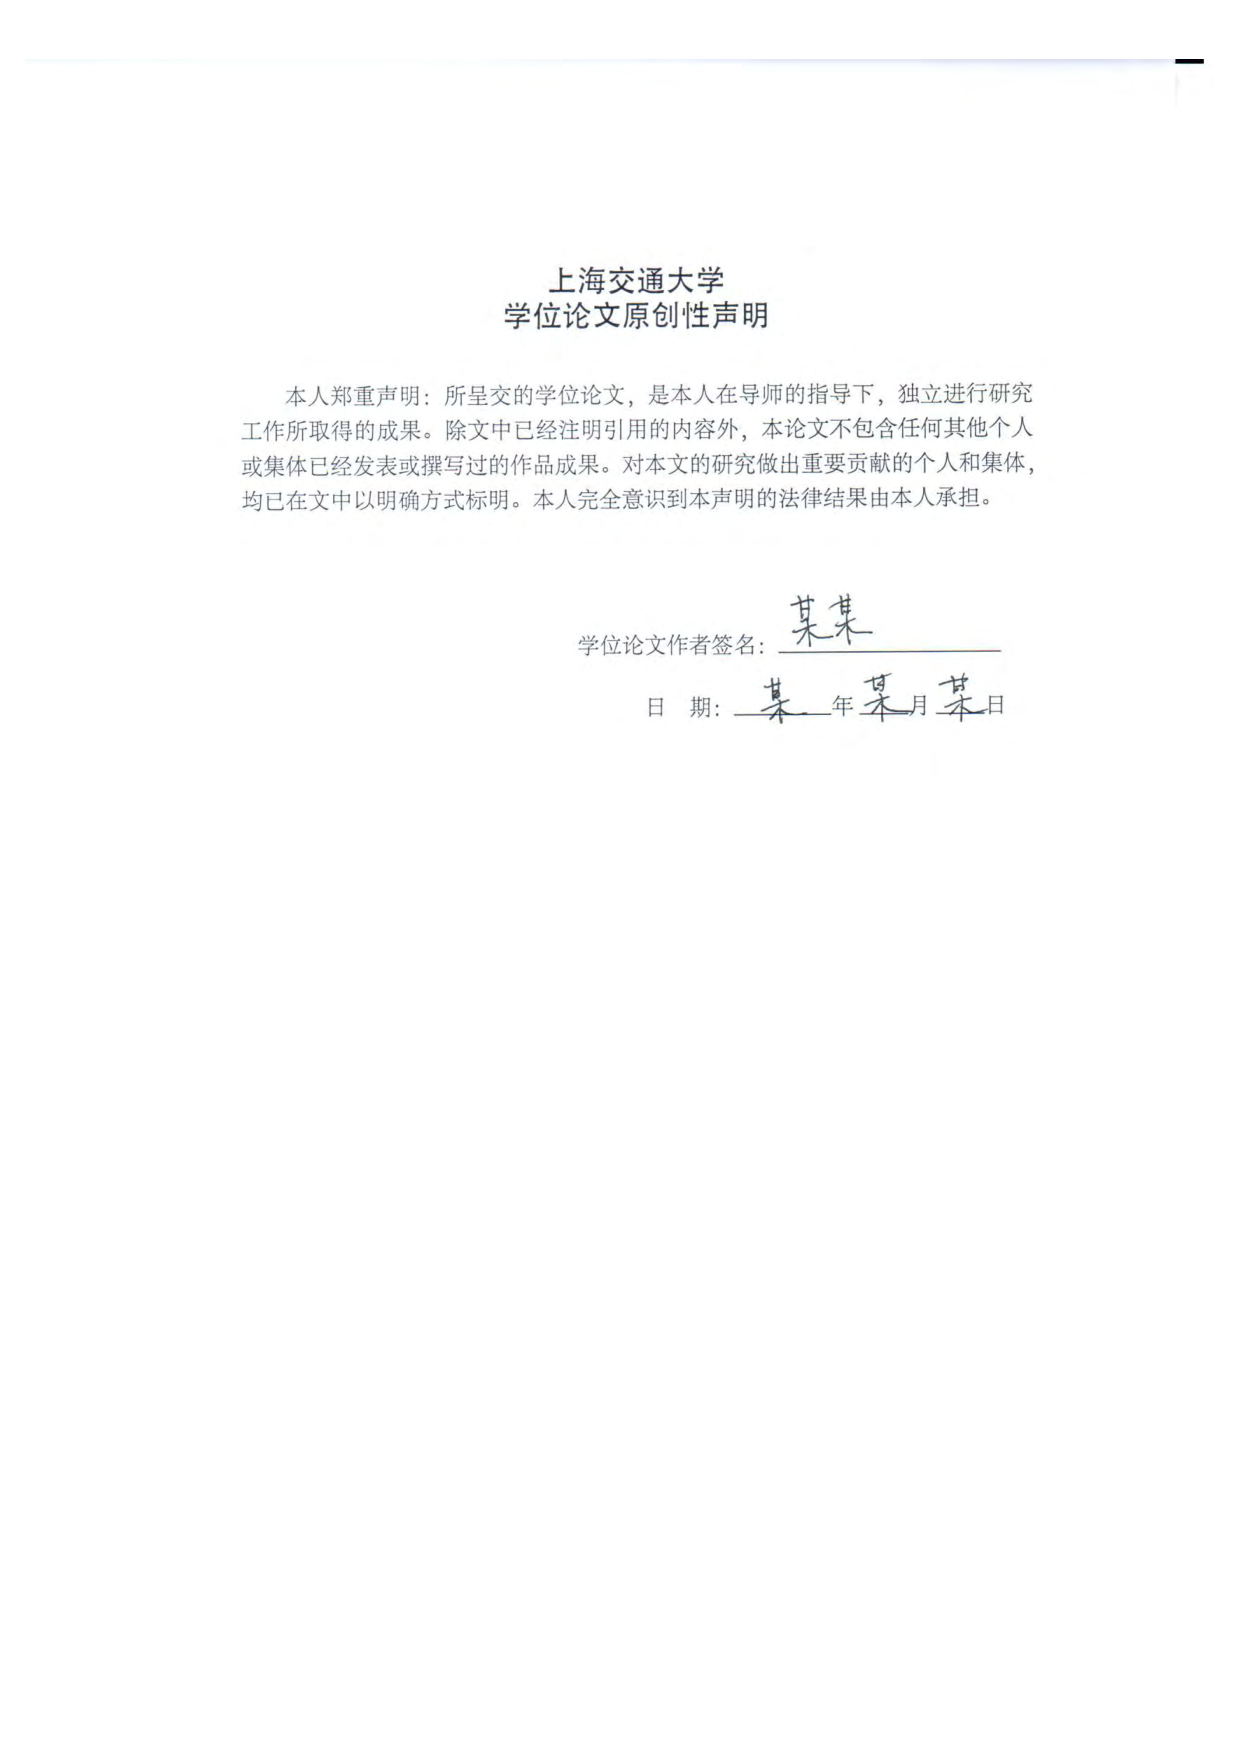
\includepdf{pdf/original.pdf}
	\cleardoublepage
	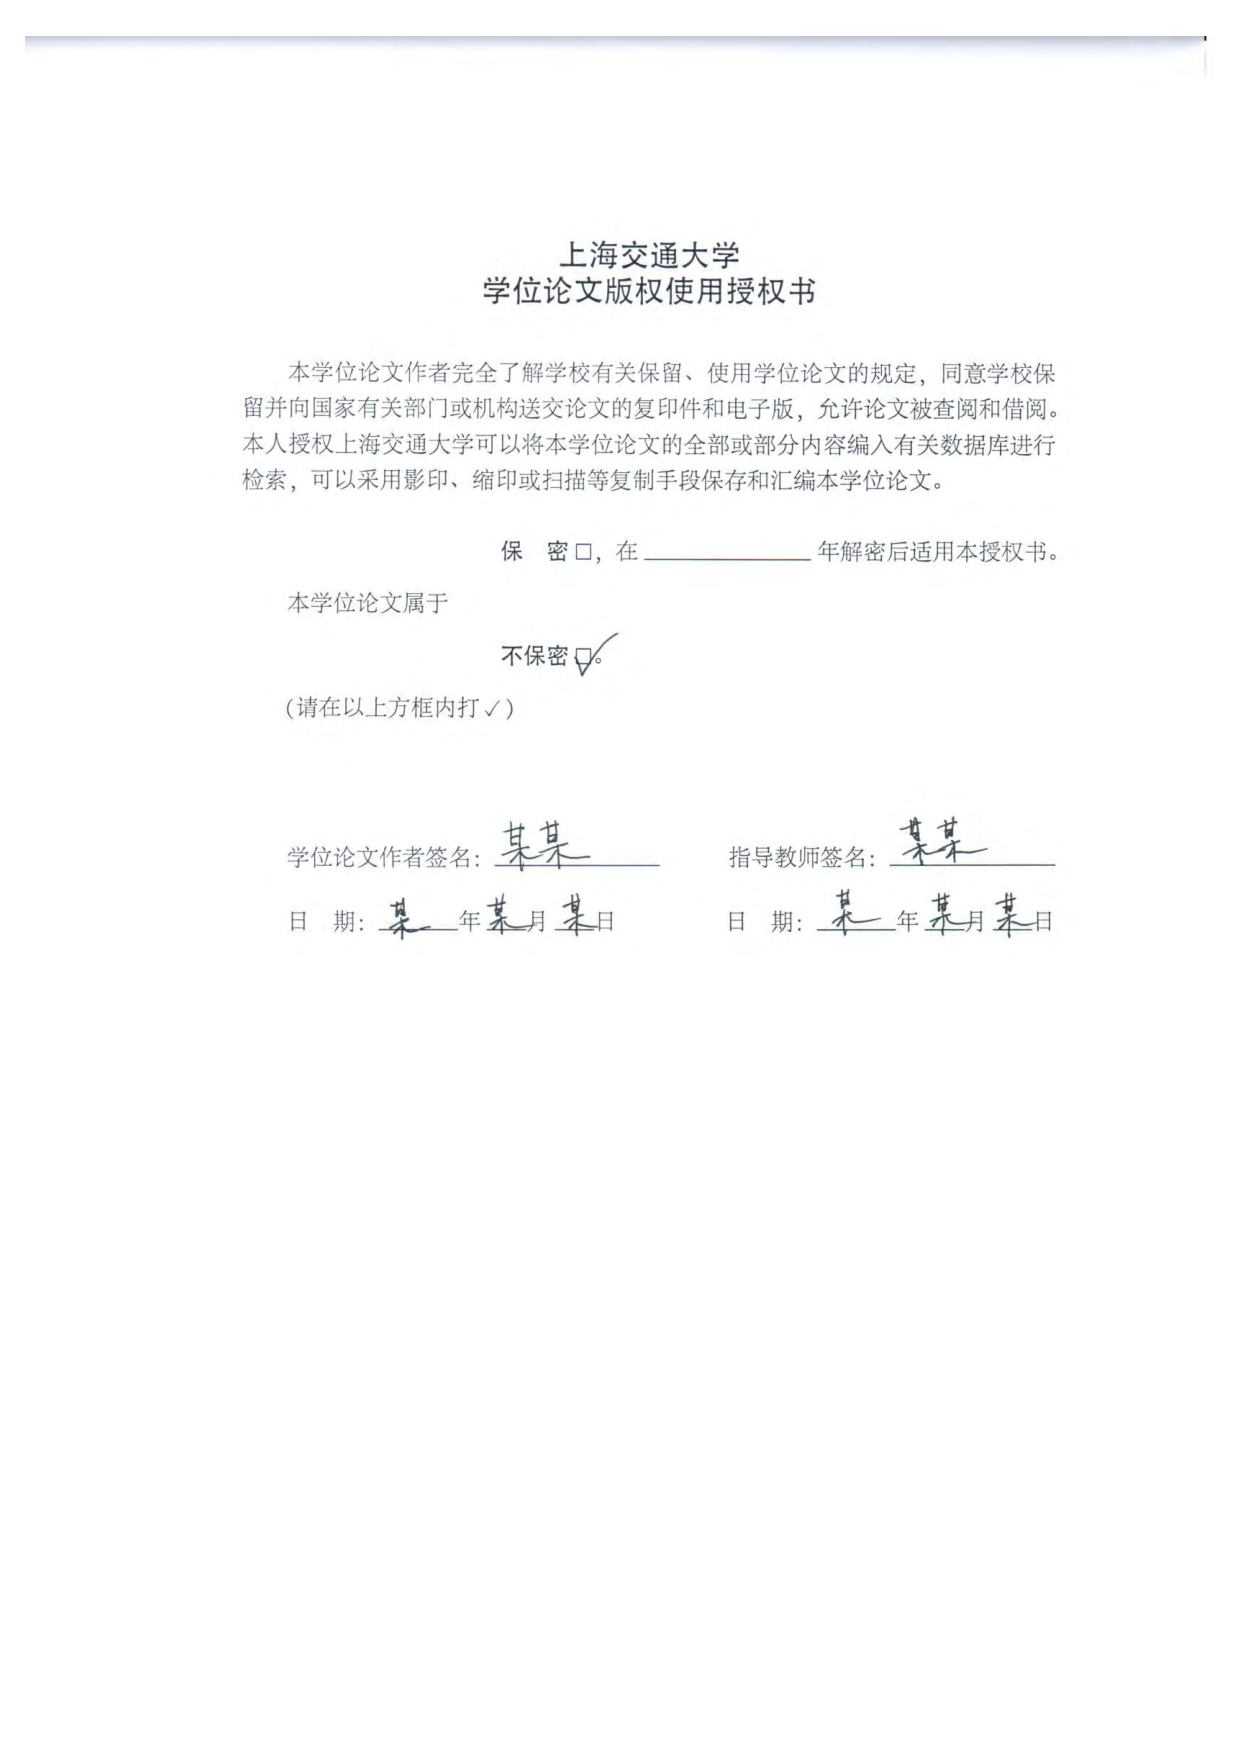
\includepdf{pdf/authorization.pdf}
	\cleardoublepage
\else
	\makeDeclareOriginal
	\makeDeclareAuthorization
\fi
\makeatother


\frontmatter 	% 使用罗马数字对前言编号

%% 摘要
\pagestyle{main}
%# -*- coding: utf-8-unix -*-
%%==================================================
%% abstract.tex for SJTU Master Thesis
%%==================================================

\begin{abstract}
时钟同步问题来源于工业中分布式系统的发展和实时性任务的需求,核心问题是通过同步方法来实现各个子系统之间的时钟一致性,传统的GPS同步方法和NTP(网络时钟同步协议)等协议由于价格昂贵、同步精度差等原因满足不了工业需求,IEEE1588精确时钟同步协议协议是目前时钟同步领域最好的同步方法,不过其在实际使用中由于链路延时等因素影响难以达到亚微秒甚至纳秒同步精度以及无法保证从时钟的稳定性。

本文从统计角度出发,对链路延时、时钟伺服系统及时钟频率漂移补偿进行深入研究,旨在提供一种系统性的统计方法来提高IEEE1588时钟同步系统精度及稳定性,主要工作如下:

(1) 通过对链路延时成分进行数学特性分析,并从统计角度提出动态阈值法与基于固定时间窗的实时监控算法等以提高同步精度;

(2) 在时钟伺服系统中,针对链路时延的阶跃突变干扰采用多模型PID控制策略,以优化从时钟的稳定性,减少从时钟的频繁抖动以保证整个系统的平稳运行;

(3) 对于时钟频率漂移问题,通过监测PTP报文样本是否发生链路堵塞等来进行报文过滤,只选取正常链路传输的PTP样本来进行校正,从而提高频率偏差计算的准确度;

(4) 通过对比边界时钟与透明时钟差异性来对统计算法进行调整,以使本文所提算法能够应用到透明时钟场合中;

(5) 通过stateflow时钟同步仿真系统进行仿真分析。仿真结果表明上述算法不仅能够提高时钟同步系统对多种链路延时抖动的适应性,还能提高整个系统的同步精度和稳定性。

\keywords{\large 时钟同步 \quad 统计算法 \quad 频率补偿 \quad 时钟伺服系统 \quad  \quad stateflow}
\end{abstract}

\begin{englishabstract}

Time synchronization problem originates from the requirement of developing distributed system and real-time tasks. The core problem is to achieve the time consistency among all the subsystems through time-synchronization method. The traditional GPS method and NTP protocol are not able to meet current industrial demand due to their high-cost and unpredictable message latency. Currently, IEEE1588 protocol is the best choice for time-synchronization problem, However, it often cannot achieve the precision level of sub-microsecond or nanosecond and it's not able to guarantee the stability of slave clock in the industrial reality.

From the perspective of mathematical statistics, the objective of this paper is to promote a systematically statistical method to improve the time-synchronization precision and stability. The contributions are shown in the following.

(1) Through the mathematical analysis for transmitting message latency, I decomposed latency into inherent jitter, temporary latency mutation and persistent latency change. In order to improve accuracy, dynamic threshold method and fixed-window real-time detection method are promoted.

(2) In clock servo system, multi-model PID controller strategy is promoted for improving the slave-clock stability when step-mutation occurs. So slave clock system will become more smooth due to the less jitter.

(3) By filtering PTP messages based on the detection of link blocking, qualified PTP messages will be choosed for calcuation of master-to-slave frequency offset.

(4) By comparing boundary-clock with transparent-clock, the statistics methods are promoted in order to make our statistical methods able to be applied into the occasion of transparent-clock device.

(5) Based on stateflow time-synchronization simulation system, all the promoted methods above get validated and verified. The simulation results show us those methods above can improve the adaptive ability of time-synchronization system for multiple types of latency changes, and the synchronization precision and stability of whole system as well.

\englishkeywords{\large clock synchronization,  statistical method, frenquency compensation, clock servo, stateflow}
\end{englishabstract}



%% 目录、插图目录、表格目录
\tableofcontents
\listoffigures
\addcontentsline{toc}{chapter}{\listfigurename} %将插图目录加入全文目录
\listoftables
\addcontentsline{toc}{chapter}{\listtablename}  %将表格目录加入全文目录
% \listofalgorithms
% \addcontentsline{toc}{chapter}{代码索引}  %将表格目录加入全文目录

%# -*- coding: utf-8-unix -*-
\chapter{主要符号对照表}
\label{chap:symb}

\begin{longtable}{rl}
$\epsilon$     & 介电常数 \\
 $\mu$ 		& 磁导率 \\
 $\epsilon$     & 介电常数 \\
 $\mu$ 		& 磁导率 \\
 $\epsilon$     & 介电常数 \\
 $\mu$ 		& 磁导率 \\
 $\epsilon$ 	& 介电常数 \\
 $\mu$ 		& 磁导率 \\
 $\epsilon$     & 介电常数 \\
 $\mu$ 		& 磁导率 \\
 $\epsilon$     & 介电常数 \\
 $\mu$ 		& 磁导率 \\
 $\epsilon$     & 介电常数 \\
 $\mu$ 		& 磁导率 \\
 $\epsilon$ 	& 介电常数 \\
 $\mu$ 		& 磁导率 \\
 $\epsilon$     & 介电常数 \\
 $\mu$ 		& 磁导率 \\
 $\epsilon$     & 介电常数 \\
 $\mu$ 		& 磁导率 \\
 $\epsilon$     & 介电常数 \\
 $\mu$ 		& 磁导率 \\
 $\epsilon$ 	& 介电常数 \\
 $\mu$ 		& 磁导率 \\
 $\epsilon$     & 介电常数 \\
 $\mu$ 		& 磁导率 \\
 $\epsilon$     & 介电常数 \\
 $\mu$ 		& 磁导率 \\
 $\epsilon$     & 介电常数 \\
 $\mu$ 		& 磁导率 \\
 $\epsilon$ 	& 介电常数 \\
 $\mu$ 		& 磁导率 \\
 $\epsilon$     & 介电常数 \\
 $\mu$ 		& 磁导率 \\
 $\epsilon$     & 介电常数 \\
 $\mu$ 		& 磁导率 \\
 $\epsilon$     & 介电常数 \\
 $\mu$ 		& 磁导率 \\
 $\epsilon$ 	& 介电常数 \\
 $\mu$ 		& 磁导率 \\
 $\epsilon$     & 介电常数 \\
 $\mu$ 		& 磁导率 \\
 $\epsilon$     & 介电常数 \\
 $\mu$ 		& 磁导率 \\
 $\epsilon$     & 介电常数 \\
 $\mu$ 		& 磁导率 \\
 $\epsilon$ 	& 介电常数 \\
 $\mu$ 		& 磁导率 \\
 $\epsilon$     & 介电常数 \\
 $\mu$ 		& 磁导率 \\
 $\epsilon$     & 介电常数 \\
 $\mu$ 		& 磁导率 \\
 $\epsilon$     & 介电常数 \\
 $\mu$ 		& 磁导率 \\
\end{longtable}
 % 主要符号、缩略词对照表

\mainmatter	% 使用阿拉伯数字对正文编号

%% 正文内容
\pagestyle{main}
\include{tex/chapter01}
\include{tex/chapter02}
\include{tex/chapter03}
%# -*- coding: utf-8-unix -*-
%%==================================================
%% conclusion.tex for SJTUThesis
%% Encoding: UTF-8
%%==================================================

\begin{summary}
研究生期间,在导师带领下,本人开始逐步接触时钟同步技术和IEEE1588精密时钟同步协议。在了解中发现,目前工业领域越来越多的应用了IEEE1588精密时钟同步协议来提高分布式系统的同步性能,所以也在研究学习中对时钟同步技术和IEEE1588协议本身产生兴趣。然后通过不断的阅读各种文献和深入阅读IEEE1588协议内容,对时钟同步技术有了全面的了解。

不过,慢慢就发现了IEEE1588精密时钟同步协议在实际应用中仍然存在的很多缺陷和问题。正是这些问题的存在导致了实际的运行效果不尽如人意,其同步精度也往往很难达到理想的目标。因此,决定着手深入研究这些问题的根源及其解决方案。

在导师的指引下,文章中创新性地从数学统计角度来深入分析这些问题,并且提出了一套自己的解决方案,这一套统计算法覆盖了报文固有抖动、排队堵塞等导致的暂时性时延突变、拓扑结构变化导致的持久性时延变化和从时钟频率漂移等多种破坏同步精度的因素。最后,通过搭建的stateflow仿真平台上对所提算法进行验证,可以发现这些算法不仅能有效提高系统的同步精度,还能改善同步系统应对复杂工业环境的稳定性和自适应性。

然后,通过这篇论文的撰写,又重新梳理了之前的思路,并试图以尽可能准确的语言和描述把之前的研究工作及成果展示给大家。同时,也将研究过程进行记录,以方面后续的研究人员在此基础上能够继续探究,不断改良时钟同步系统的精度,使得IEEE1588协议能够发挥其理想的效果,具备更大的实际应用价值。

最后,通过对时钟同步技术的研究,我也培养了自身的科研习惯,能够从更加理性的角度去思考问题,也学会了通过阅读国内外文献来扩展自己的视野和优化自己的思维方式。另外,这个过程也让我感受到了科研的魅力,受益匪浅。相信以后能够继续保持这种谨慎认真的态度来面对未来的工作和学习。

\end{summary}


\appendix	% 使用英文字母对附录编号,重新定义附录中的公式、图图表编号样式
\renewcommand\theequation{\Alph{chapter}--\arabic{equation}}	
\renewcommand\thefigure{\Alph{chapter}--\arabic{figure}}
\renewcommand\thetable{\Alph{chapter}--\arabic{table}}
\renewcommand\thealgorithm{\Alph{chapter}--\arabic{algorithm}}

%% 附录内容,本科学位论文可以用翻译的文献替代。
%# -*- coding: utf-8-unix -*-
\chapter{搭建模板编译环境}

\section{安装TeX发行版}

\subsection{Mac OS X}

Mac用户可以从MacTeX主页\footnote{\url{https://tug.org/mactex/}}下载MacTeX 2015。
也可以通过brew包管理器\footnote{\url{http://caskroom.io}}安装MacTeX 2015。

\begin{lstlisting}[basicstyle=\small\ttfamily, numbers=none]
brew cask install mactex
\end{lstlisting}

\subsection{Linux}

建议Linux用户使用TeXLive主页\footnote{\url{https://www.tug.org/texlive/}}的脚本来安装TeXLive 2015。
以下命令将把TeXLive发行版安装到当前用户的家目录下。
若计划安装一个供系统上所有用户使用的TeXLive,请使用root账户操作。

\begin{lstlisting}[basicstyle=\small\ttfamily, numbers=none]
wget http://mirror.ctan.org/systems/texlive/tlnet/install-tl-unx.tar.gz
tar xzvpf install-tl-unx.tar.gz
cd install-tl-20150411/
./install-tl
\end{lstlisting}

\section{安装中文字体}

\subsection{Mac OS X、Deepin}

Mac和Deepin用户双击字体文件即可安装字体。

\subsection{RedHat/CentOS用户}

RedHat/CentOS用户请先将字体文件复制到字体目录下,调用fc-cache刷新缓存后即可在TeXLive中使用新字体。

\begin{lstlisting}[basicstyle=\small\ttfamily, numbers=none]
mkdir ~/.fonts
cp *.ttf ~/.fonts				# 当前用户可用新字体
cp *.ttf /usr/share/fonts/local/	# 所有用户可以使用新字体
fc-cache -f
\end{lstlisting}


%# -*- coding: utf-8-unix -*-
%% app2.tex for SJTU Master Thesis
%% based on CASthesis
%% modified by wei.jianwen@gmail.com
%% version: 0.3a
%% Encoding: UTF-8
%% last update: Dec 5th, 2010
%%==================================================

\chapter{Maxwell Equations}

选择二维情况,有如下的偏振矢量:
\begin{subequations}
  \begin{eqnarray}
    {\bf E}&=&E_z(r,\theta)\hat{\bf z} \\
    {\bf H}&=&H_r(r,\theta))\hat{ \bf r}+H_\theta(r,\theta)\hat{\bm
      \theta}
  \end{eqnarray}
\end{subequations}
对上式求旋度:
\begin{subequations}
  \begin{eqnarray}
    \nabla\times{\bf E}&=&\frac{1}{r}\frac{\partial E_z}{\partial\theta}{\hat{\bf r}}-\frac{\partial E_z}{\partial r}{\hat{\bm\theta}}\\
    \nabla\times{\bf H}&=&\left[\frac{1}{r}\frac{\partial}{\partial
        r}(rH_\theta)-\frac{1}{r}\frac{\partial
        H_r}{\partial\theta}\right]{\hat{\bf z}}
  \end{eqnarray}
\end{subequations}
因为在柱坐标系下,$\overline{\overline\mu}$是对角的,所以Maxwell方程组中电场$\bf E$的旋度:
\begin{subequations}
  \begin{eqnarray}
    &&\nabla\times{\bf E}=\mathbf{i}\omega{\bf B} \\
    &&\frac{1}{r}\frac{\partial E_z}{\partial\theta}{\hat{\bf
        r}}-\frac{\partial E_z}{\partial
      r}{\hat{\bm\theta}}=\mathbf{i}\omega\mu_rH_r{\hat{\bf r}}+\mathbf{i}\omega\mu_\theta
    H_\theta{\hat{\bm\theta}}
  \end{eqnarray}
\end{subequations}
所以$\bf H$的各个分量可以写为:
\begin{subequations}
  \begin{eqnarray}
    H_r=\frac{1}{\mathbf{i}\omega\mu_r}\frac{1}{r}\frac{\partial
      E_z}{\partial\theta } \\
    H_\theta=-\frac{1}{\mathbf{i}\omega\mu_\theta}\frac{\partial E_z}{\partial r}
  \end{eqnarray}
\end{subequations}
同样地,在柱坐标系下,$\overline{\overline\epsilon}$是对角的,所以Maxwell方程组中磁场$\bf H$的旋度:
\begin{subequations}
  \begin{eqnarray}
    &&\nabla\times{\bf H}=-\mathbf{i}\omega{\bf D}\\
    &&\left[\frac{1}{r}\frac{\partial}{\partial
        r}(rH_\theta)-\frac{1}{r}\frac{\partial
        H_r}{\partial\theta}\right]{\hat{\bf
        z}}=-\mathbf{i}\omega{\overline{\overline\epsilon}}{\bf
      E}=-\mathbf{i}\omega\epsilon_zE_z{\hat{\bf z}} \\
    &&\frac{1}{r}\frac{\partial}{\partial
      r}(rH_\theta)-\frac{1}{r}\frac{\partial
      H_r}{\partial\theta}=-\mathbf{i}\omega\epsilon_zE_z
  \end{eqnarray}
\end{subequations}
由此我们可以得到关于$E_z$的波函数方程:
\begin{eqnarray}
  \frac{1}{\mu_\theta\epsilon_z}\frac{1}{r}\frac{\partial}{\partial r}
  \left(r\frac{\partial E_z}{\partial r}\right)+
  \frac{1}{\mu_r\epsilon_z}\frac{1}{r^2}\frac{\partial^2E_z}{\partial\theta^2}
  +\omega^2 E_z=0
\end{eqnarray}

%# -*- coding: utf-8-unix -*-
\chapter{从 \CJKLaTeX 转向 \XeTeX }
\label{chap:whydvipdfm}

我习惯把v0.2a使用dvipdfmx编译的硕士学位论文模板称为“ \CJKLaTeX 模板”,而这个使用 \XeTeX 引擎(xelatex程序)处理的模板则被称为“{\XeTeX/\LaTeX}模板”。
从 \CJKLaTeX 模板迁移到{\XeTeX\LaTeX}模板的好处有下:
\begin{enumerate}
\item[\large\smiley] 搭建 \XeTeX 环境比搭建 \CJKLaTeX 环境更容易;
\item[\large\smiley] 更简单的字体控制;
\item[\large\smiley] 完美支持PDF/EPS/PNG/JPG图片,不需要“bound box(.bb)”文件;
\item[\large\smiley] 支持OpenType字体的复杂字型变化功能;
\end{enumerate}

当然,这也是有代价的。由于 \XeTeX 比较新,在我看来,使用 \XeTeX 模板所必须付出的代价是:

\begin{enumerate}
\item[\large\frownie] 必须把你“古老的” \TeX 系统更新为较新的版本。TeXLive 2012和CTeX 2.9.2能够编译这份模板,而更早的版本则无能为力。
\item[\large\frownie] 需要花一些时间把你在老模板上的工作迁移到新模板上。
\end{enumerate}

第一条就看你如何取舍了,新系统通常意味着更好的兼容性,值得升级。而转换模板也不是什么特别困难的事情,可以这样完成:

\begin{enumerate}
\item 备份你要转换的源文件,以防你的工作成果丢失;
\item 将你原来的tex以及bib文件另存为UTF-8编码的文件。iconv、vim、emacs、UEdit等等工具都可以完成。WinEdt对文件编码识别功能很差(到了v6.0还是如此),不推荐作为字符编码转换工具;
\item 将diss.tex导言区中的内容替换为XeTeX模板diss.tex导言区的内容;
\item 将你对原先导言区的修改,小心翼翼地合并到新的导言区中;
\item 使用XeTeX模板中的GBT7714-2005NLang.bst替换原有的bst文件,新的bst文件只是将字符编码转换为UTF-8;
\item 删除bouding box文件;
\item 使用本文\ref{sec:process}介绍的方法,重新编译文档;
\end{enumerate}


%# -*- coding: utf-8-unix -*-
\chapter{模板更新记录}
\label{chap:updatelog}

\textbf{2015年6月19日} v0.9发布,适配ctex 2.x宏包,需要使用TeXLive 2015编译。

\textbf{2015年3月15日} v0.8发布,使用biber/biblatex组合替代 \BibTeX ,带来更强大稳定的参考文献处理能力;添加enumitem宏包增强列表环境控制能力;完善宏包文字描述。

\textbf{2015年2月15日} v0.7发布,增加盲审选项,调用外部工具插入扫描件。

\textbf{2015年2月14日} v0.6.5发布,修正一些小问题,缩减git仓库体积,仓库由sjtu-thesis-template-latex更名为SJTUThesis。

\textbf{2014年12月17日} v0.6发布,学士、硕士、博士学位论文模板合并在了一起。

\textbf{2013年5月26日} v0.5.3发布,更正subsubsection格式错误,这个错误导致如"1.1 小结"这样的标题没有被正确加粗。

\textbf{2012年12月27日} v0.5.2发布,更正拼写错误。在diss.tex加入ack.tex。

\textbf{2012年12月21日} v0.5.1发布,在 \LaTeX 命令和中文字符之间留了空格,在Makefile中增加release功能。

\textbf{2012年12月5日} v0.5发布,修改说明文件的措辞,更正Makefile文件,使用metalog宏包替换xltxtra宏包,使用mathtools宏包替换amsmath宏包,移除了所有CJKtilde(\verb+~+)符号。

\textbf{2012年5月30日} v0.4发布,包含交大学士、硕士、博士学位论文模板。模板在\href{https://github.com/weijianwen/sjtu-thesis-template-latex}{github}上管理和更新。

\textbf{2010年12月5日} v0.3a发布,移植到 \XeTeX/\LaTeX 上。

\textbf{2009年12月25日} v0.2a发布,模板由CASthesis改名为sjtumaster。在diss.tex中可以方便地改变正文字号、切换但双面打印。增加了不编号的一章“全文总结”。
添加了可伸缩符号(等号、箭头)的例子,增加了长标题换行的例子。

\textbf{2009年11月20日} v0.1c发布,增加了Linux下使用ctex宏包的注意事项、.bib条目的规范要求,
修正了ctexbook与listings共同使用时的断页错误。

\textbf{2009年11月13日} v0.1b发布,完善了模板使用说明,增加了定理环境、并列子图、三线表格的例子。

\textbf{2009年11月12日} 上海交通大学硕士学位论文 \LaTeX 模板发布,版本0.1a。



\backmatter	% 文后无编号部分 

%% 参考资料
\printbibliography[heading=bibintoc]

%% 致谢、发表论文、申请专利、参与项目、简历
%% 用于盲审的论文需隐去致谢、发表论文、申请专利、参与的项目
\makeatletter
\ifsjtu@review\relax\else
  %# -*- coding: utf-8-unix -*-
\begin{thanks}

在交大研究生的这两年时间里,我从一名从没接触过科研的普通学生起步,开始接触交大优秀的教师,并在研一期间学习了非常多自己感兴趣的知识,而每一堂课的老师都能够耐心回答我所提出的疑惑,使得本人的知识面有了非常大的拓宽。所以我很感谢交大有一批优秀的教师为我们传道解惑。

进入实验室后,开始跟随导师完成实验室的项目,依次接触过软件验证、核电电路图绘制和时钟同步技术研究等多个工作。在这些工作中,导师通过不断指导给予了我很多帮助,也让我从一名初学者逐渐学习提高。尤其是在时钟同步技术方面的深入研究历程极大提高了我的科研能力,让我感受到了作为一名科研工作者应有的认真和谨慎。所以非常感谢导师对我的耐心传授和方向指引,使得我真正感受到作为一名研究生的价值。

然后,还要感谢父母在读研期间对自己的关心和鼓励,尤其是当自己生病时陪伴左右。这些都是本人不断前进的动力来源。另外,实验室的师兄弟们也给予了我很多的关心和帮助,我也要感谢他们对本人的照顾和帮助。

最后,感谢交大这所学校,本人在这里感受到了一所综合学府的学术、上进和踏实,也在这里完成了本科生到研究生的蜕变。

无论是从心智还是情感,这里的收获都将让我受益匪浅。

感谢!
\end{thanks}
 	  %% 致谢
  %# -*- coding: utf-8-unix -*-
%%==================================================
%% pub.tex for SJTUThesis
%% Encoding: UTF-8
%%==================================================

\begin{publications}{99}
    \item\textsc{第一作者}. {统计方法在IEEE1588时钟同步协议中的应用}. 化工自动化及仪表, 2015.07.
\end{publications}
	  %% 发表论文
  %# -*- coding: utf-8-unix -*-
\begin{patents}{99}
    \item 第一发明人,“永动机”,专利申请号202510149890.0
\end{patents}
	  %% 申请专利
  %# -*- coding: utf-8-unix -*-
%%==================================================
%% projects.tex for SJTUThesis
%% Encoding: UTF-8
%%==================================================

\begin{projects}{99}
    \item 973项目“XXX”
    \item 自然基金项目“XXX”
    \item 国防项目“XXX”
\end{projects}
  %% 参与的项目
% \include{tex/resume}	  %% 各人简历
\fi
\makeatother

\end{document}
